
	\begin{frame}{3.3 패널존}
	\textbf{3.3.1 일반사항}
	
	이 절은 패널존의 불균형 모멘트에 의해 전단력이 유발되는 기둥의 패널존에 적용한다.  
	
	\textbf{3.3.2 패널존의 강성}
		
	선형동적절차를 위한 패널존의 강성은 구조역학 원칙에 기반하여 $\ulcorner$건축물 강구조 설계기준 (KDS 41 31 00:2019)$\lrcorner$에 따라 산정하며, 다음에 따른다. 
	
	\begin{enumerate}
		\item[(1)] 패널존의 강성을 고려해야 할 경우, 해석모델에 패널존 요소를 추가하여 해석하거나 \texttt{(3.3.5 패널존 모델링, 후술)} 또는 패널존의 변형이 반영되도록 보 부재의 휨강성을 조정하여 해석할 수 있다.  
		\item[(2)] 패널존의 예상전단강도가 기둥--보 접합면에서 보의 휨강도 이상이며 패널존의 강성이 보 휨강성의 10배를 초과할 경우, 패널존은 기둥 중심선에서  기둥--보 접합면까지를 가체 오프셋(rigid-end offset)으로 모델링한다. 
		\item[(3)] 위 (1)과 (2)의 적용이 어려운 경우 부재 중심간 거리를 사용한 근사 골조해석모델을 사용할 수 있다. 
	\end{enumerate}
	\end{frame}
	


	\begin{frame}{3.3 패널존}

	\textbf{3.3.3 패널존의 강도}

3.3.3.1 선형동적절차	

선형동적절차를 위한 패널존의 강성은 구조역학 원칙에 기반하여 $\ulcorner$건축물 강구조 설계기준 (KDS 41 31 00:2019)$\lrcorner$에 따라 산정한다. 

3.3.3.2 비선형정적 및 동적절차

	\begin{enumerate}
		\item[(1)] 비선형정적절차의 경우, 표 3-3에 따라 그림 1-1과 같은 비선형 부재력--변형 관계를 결정한다. 패널존의 예상부재강도 $Q_{CE}$는 선형절차와 동일한 값을 사용한다. 
		\item[(2)] 비선형동적절차의 이력거동모델링은 실험이나 정밀해석을 통해 얻어진 관계를 사용할 수 있으며, 포락곡선으로는 표 3-3에 사용된 모델을 적용할 수 있다. 
		\begin{figure}
			\centering
			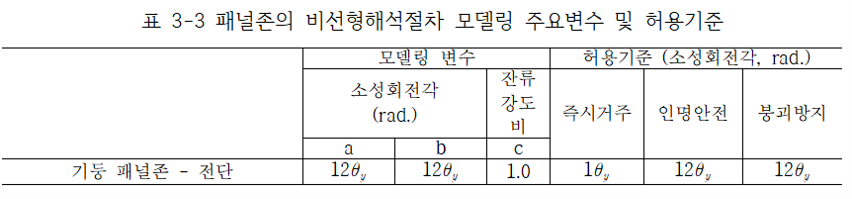
\includegraphics[width=.89\textwidth]{table05}
		\end{figure}
	\end{enumerate}

	\end{frame}	
	
	

	\begin{frame}{3.3 패널존}

	\textbf{3.3.4 패널존의 허용기준}

3.3.4.1 선형동적절차

선형동적절차를 위한 패널존의 허용기준은 표 3-4에 따르며, 다음의 사항을 고려한다. 

	\begin{enumerate}[label=\large\protect\textcircled{\small\arabic*}]
		\item 패널존 전단은 변형지배거동으로 보고 패널존 예상전단강도 $Q_{CE}$를 산정한다. 
		\item 다음 조건을 만족하지 못할 경우 표 3-4의 $m$계수 값에 0.8을 곱하여 평가한다. 
		\[0.6 \geq \frac{V_{PZ}}{V_y} \geq 0.9\]
		\noindent 여기서 $V_y$는 패널존의 항복전단력($0.55F_{yec}d_ct_{cw}$)이고 $V_{PZ}$는 접합부 위험단면에 힌지발생 시 패널존에 작용하는 전단력의 크기로 아래와 같이 산정한다. 
		\[V_{PZ} = \sum \frac{M_y^{beam}}{d_b}\Big(\frac{L}{L-d_c}\Big)\Big(\frac{h - d_b}{h}\Big)\]
	\end{enumerate}		
	
	\end{frame}
	
	\begin{frame}{3.3 패널존}

	\textbf{3.3.4 패널존의 허용기준}
		
3.2.4.2 비선형 정적 및 동적절차	

	\begin{enumerate}
		\item[(1)] 패널존 전단은 변형지배거동으로 보고 패널존 예상전단강도 $Q_{CE}$를 산정한다.   
		\item[(2)] 위 조건을 만족하지 못할 경우 표 3-3에 의한 허용소성회전각의 값에 0.8을 곱하여 평가한다.  
	\end{enumerate}
\end{frame}	
	
	
	
	\begin{frame}{3.3 패널존}

	\textbf{3.3.5 패널존의 모델링}
	
	\begin{enumerate}
		\item[(1)] 패널존의 소요전단력이 패널존의 항복강도를 초과할 경우 패널존 비탄성응답은 그림 3-3과 같은 전단력과 전단변형에 대한 삼선형 관계를 사용한다. 
		\item[(2)] 그림 3-3에서 $V_{y,PZ}$는 전단항복강도, $V_{p,PZ}$는 전단소성강도이고, $\gamma_{y,PZ}$와 $\gamma_{p,pz}$는 각각 전단항복변형각과 전단소성변형각이다. 패널존의 탄성전단강성 $K_{e,PZ}$는 다음 식으로 산정한다. 
		\[K_{e,PZ} = GA_{z,PZ}\]
		\noindent 여기서 $G$는 강재 전단탄성계수이고, $A_{s,PZ}$는 웨브 단면적으로, 기둥 춤에 더블러플레이트를 포함한 웨브의 두께를 반영한다. 
		\begin{figure}
			\centering
			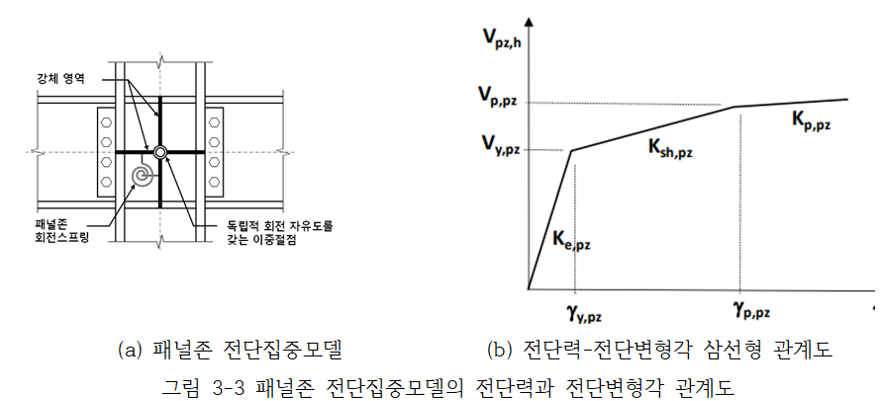
\includegraphics[width=0.5\textwidth]{image3-3}
		\end{figure}		
	\end{enumerate}
	\end{frame}
	
	
	\begin{frame}{3.3 패널존}

	\textbf{3.3.5 패널존의 모델링}
	
	\begin{enumerate}
		\item[(3)] 패널존의 전단소성강도는 다음과 같이 산정한다. 
		\[R_n = 0.6F_yd_ct_w\Big(1 + \frac{3b_{cf}t_{cf}^2}{d_bd_ct_w}\Big)~~~\alpha P_r \leq 0.75 P_y\]		
		\[R_n = 0.6F_yd_ct_w\Big(1 + \frac{3b_{cf}t_{cf}^2}{d_bd_ct_w}\Big)\Big(1.9-\frac{1.2\alpha P_r}{P_y}\Big)~~~\alpha P_r > 0.75 P_y\]		
		\item[(4)] 변형경화기울기 $K_{sh,PZ}$를 정의하는 전단소성변형각 $\gamma_{p,PZ}$는 전단항복변형각 $\gamma_{y,PZ}$ 값의 네 배를 적용한다. 패널존 변형에 의한 킹크(Kink) 변형에 의해 보--기둥 용접부 파단이 우려되는 경우, 파단을 제어하기 위한 변형한계로서 패널존 전단소성변형각 $\gamma_{p,PZ}$는 다음과 같이 산정한다. 
		\[\gamma_{p,PZ} = \frac{0.475F_{yc}}{E}\Big(\frac{d_b}{t_{fc}}+3.45\frac{t_{fc}}{d_b}\Big)\]
		\noindent 여기서 $F_{yc}$는 기둥 플랜지의 강재 항복강도, $E$는 강재탄성계수, $d_b$는 보의 춤이고, $t_{fc}$는 기둥 플랜지 두께이다.  
	\end{enumerate}
	\end{frame}
	
	
	

	\begin{frame}{3.3 패널존}

	\textbf{3.3.5 패널존의 모델링}
	
	\begin{enumerate}
		\item[(5)] 소성기울기 $K_{p,PZ}$는 $K_{e,PZ}$의 1--2\%이다. 
		\item[(6)] 위 전단집중 모델을 소프트웨어 상에서 불균형모멘트--회전각 관계로 모델링 하는 경우, 패널존 전단력에 보의 춤을 곱하여 불균형모멘트를 산정한다. 
	\end{enumerate}
	\end{frame}